\section{Applications and Evaluation}
We evaluate our formalization and implementation of the SFT product operation across two key application domains: string sanitization and string replacement in string solving. These case studies highlight the practical value of our certified SFT product operation in real-world scenarios.
\subsection{Sanitizer}

An important application of our formalization lies in string sanitization for web applications. Sanitizers are crucial for preventing security vulnerabilities such as cross-site scripting (XSS) attacks by ensuring that user inputs are properly encoded before rendering in web browsers. Listing \ref{lst-html-encode} presents a C\# code snippet implementing an HTML encoding function—a fundamental sanitization operation. This function iterates through each character in the input string and encodes characters that are unsafe for HTML rendering.



\begin{lstlisting}[language={[Sharp]C}, caption={C\# Code for AntiXSS.EncodeHtml version 2.0.}, label={lst-html-encode}, float=htbp]
static string EncodeHtml(string t)
{
  if (t == null) { return null; }
  if (t.Length == 0) {
    return string.Empty;
  }
  StringBuilder builder = new
    StringBuilder("", t.Length * 2);
  foreach (char c in t) {
    if ((((c > ''') && (c < '{')) |$\mid\mid$|
         ((c > '@') && (c < '['))) |$\mid\mid$|
         (((c == ' ') || ((c > '/') && (c < ':'))) |$\mid\mid$|
         (((c == '.') || (c == ',')) |$\mid\mid$|
         ((c == '-') || (c == '_'))))) {
          builder.Append(c);
      }
      else {
          builder.Append("&#" +
          ((int) c).ToString() + ";");
      }
  }
  return builder.ToString();
}
\end{lstlisting}

Figure \ref{fig:html-sanitizer-sft} illustrates the SFT representation of the HTML encoding sanitizer function. The transducer accepts any input string and produces an output where safe characters are preserved using the identity function $\texttt{id}$, while unsafe characters are encoded as HTML entities. The set of safe characters is defined as $\texttt{safe\_chars} = [\texttt{' '}, \texttt{','}, \texttt{'.'}, \texttt{'-'}, \texttt{'\_'}] \cup [\texttt{'0'}-\texttt{'9'}] \cup [\texttt{'A'}-\texttt{'Z'}] \cup [\texttt{'a'}-\texttt{'z'}]$, which can be efficiently represented using the interval algebra we formalized. Unsafe characters are transformed using the encoding function $\texttt{encode}(c) = \texttt{``\&\#''} + \texttt{toString}(\texttt{ord}(c)) + \texttt{``\;''}$. When the alphabet is set to Unicode $[\mathtt{0x0000}, \mathtt{0x10FFFF}]$, the complement $\neg\texttt{safe\_chars}$ represents all Unicode characters outside the safe set, which can also be efficiently represented using our formalized interval operations.
\begin{figure}[htbp]
\centering
\begin{tikzpicture}[shorten >=1pt, node distance=2.5cm, on grid, auto]
  % States
  \node[state, initial, accepting] (q0) {$q_0$};
  \node[state] (q1) [right=3.5cm of q0] {$q_1$};
  \node[state] (q2) [below=of q0] {$q_2$};
  
  \path[->] 
    % Transition for safe characters
    (q0) edge[bend left=20] node[above,midway=1] {$\texttt{safe\_chars}, \texttt{id}$} (q1)
    % Transition for unsafe characters  
    (q0) edge[bend right=20] node[left,midway] {$\neg\texttt{safe\_chars}, \texttt{encode}$} (q2)
    % Epsilon transitions back to q0
    (q1) edge[bend left=30] node[below,midway] {$\varepsilon, \lambda\varepsilon$} (q0)
    (q2) edge[bend right=20] node[right,midway] {$\varepsilon, \lambda\varepsilon$} (q0);
\end{tikzpicture}
\caption{SFT representation of the HTML encoding sanitizer function.}
\label{fig:html-sanitizer-sft1}
\end{figure}

We evaluate the performance of our SFT product operation by computing the product of the HTML encoding sanitizer SFT with SFAs constructed from randomly generated Unicode user inputs. This experimental setup reflects realistic usage scenarios where diverse character sets and input patterns are encountered. The experimental evaluation was conducted on a laptop with an Apple M4 processor and 24 GB of memory, with a one-minute time limit per test.

Figure \ref{fig:benchmark-results} demonstrates the scalability characteristics of our SFT product implementation. The computation requires approximately 1 second for 100,000-character inputs and 10 seconds for 1,000,000-character inputs. These performance metrics confirm that our certified implementation maintains computational efficiency suitable for practical string processing applications at scale.

\begin{figure}
\centering
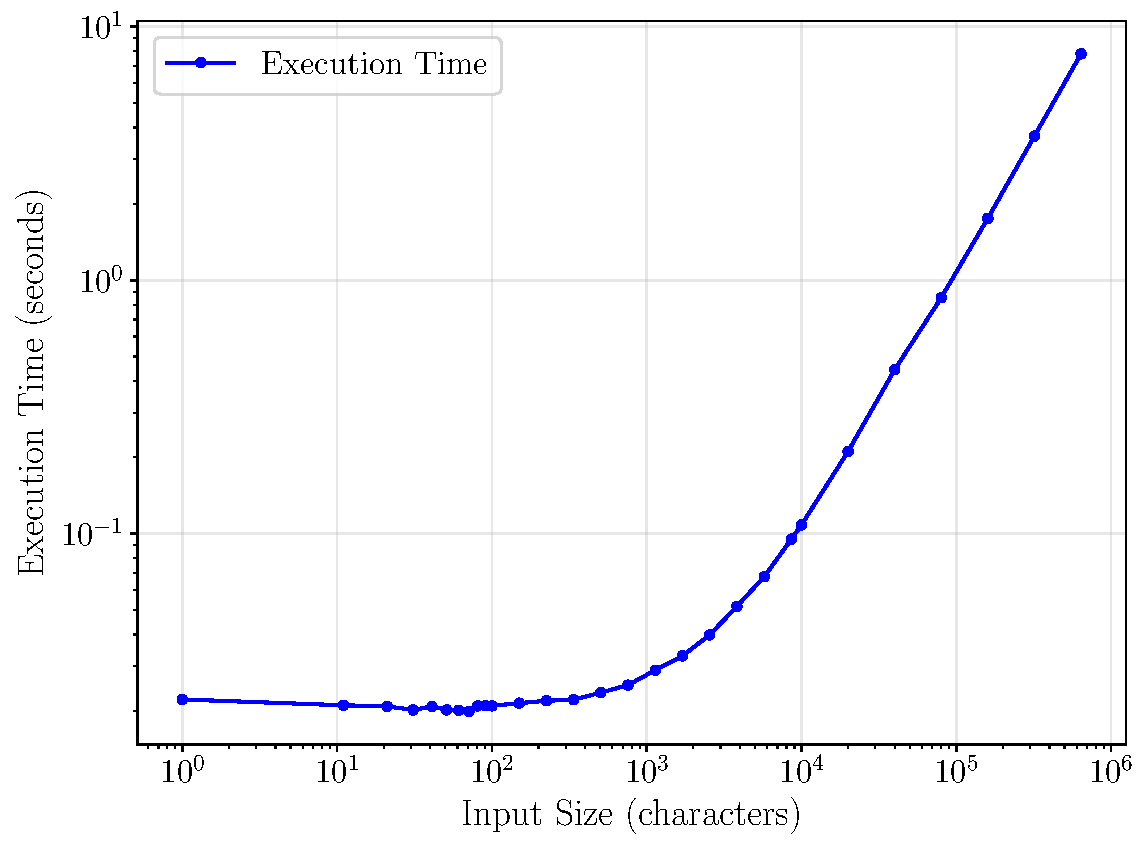
\includegraphics[scale=0.45]{benchmark_loglog.pdf}
\caption{Experimental results for the sanitizer product}
\label{fig:benchmark-results}
\end{figure}

Beyond performance evaluation, our SFT formalization also supports the formal verification of string sanitizer correctness. A sanitizer transforms user inputs into safe outputs, ensuring that the result contains no unsafe characters. However, sanitizers—like any other programs—are error-prone. Manual reviews or testing alone are often insufficient to guarantee their correctness.

Based on our formalization, we can verify sanitizers by modeling the sanitizer as an SFT and the user input as an SFA. We can also model potential attacks as SFAs that accept unsafe strings. Formally speaking, Let $\mathcal{T}$ be an SFT, $\mathcal{I}$ is the possible user inputs modeled by an SFA, and $\mathcal{A}$ is the attack SFA that accepts unsafe strings. The santizer correctness checking against the attack is to check whether the intersection of the product $\mathcal{T} \times \mathcal{I}$ and the attack SFA $\mathcal{A}$ is empty, i.e., $(\mathcal{T} \times \mathcal{I}) \cap \mathcal{A} = \emptyset$.

Moreover, santizers are usually used in combination with other sanitizers to ensure comprehensive safety. For example, the HTML encoding sanitizer can be combined with a string trimming operation to remove leading and trailing whitespace characters. For this kind of sanitizer composition, it can be modeled by our SFT product as well. Let $\mathcal{T}_1$ and $\mathcal{T}_2$ correspond to two sanitizers, and $\mathcal{T}_1$ is applied before $\mathcal{T}_2$. What we need to check is $(\mathcal{T}_2 \times (\mathcal{T}_1 \times \mathcal{I})) \cap \mathcal{A} = \emptyset$.




\begin{table}[h]
  \centering
  \small
  \setlength{\tabcolsep}{4pt} % Reduced column gap
  \begin{tabular}{p{2.2cm}ll} % Increased width for automatic line break
    \toprule
    \textbf{Attack Model} & \textbf{Verfication Result} & \textbf{Size} \\
    \midrule
    attack\_html           & GA HtmlEscape: \textbf{Unsafe} & 1/6\\
                           & Trim + GA HtmlEscape: \textbf{Safe} & 4/12 \\
                           & escapeString: \textbf{Unsafe} & 1/11 \\
                           & Trim + escapeString: \textbf{Safe} & 4/17 \\
                           & Trim + OWASP HTMLEncode: \textbf{Safe} & 4/18 \\
    \midrule
    attack\_javascript     & GA Htmlescape + GA PreEscape + & 3/20 \\
                           &  gaSnippetesc: \textbf{safe} & \\
    \midrule
    attack\_json           & Trim + GA JSONESc : \textbf{Safe} & 4/16\\
    \midrule
    attack\_xml            & Trim + GA XMLEsc: \textbf{safe} & 4/16\\
    \midrule
    attack\_ccs            & Trim + GA CleanseCSS : \textbf{Safe} & 25/46\\
    \bottomrule
  \end{tabular}
  \caption{Sanitizer verfication result}
  \label{tab:sanitizer_attack}
\end{table}

Table \ref{tab:sanitizer_attack} summarizes the verification results for various sanitizers against different attack models. The first column lists the attack models, the second column indicates whether the sanitizer is classified as safe or unsafe with respect to the attack, and the third column reports the size of the transducers used in the verification, given as [number of states/number of transitions]. For composed SFTs, the size reflects the total number of states and transitions across all SFTs.

We evaluate a range of attack models for HTML, JavaScript, JSON, XML, and CSS. Listing \ref{lst-css-attack} shows the CSS attack model, which is used to verify the corresponding sanitizer. The attack model includes comments, declaration breakers, and known dangerous tokens such as \textbf{expression(}, \textbf{@import}, \textbf{behavior:}, \textbf{-moz-binding}, and \textbf{url(} (unless the URL is separately validated). Sanitizers include GA HtmlEscape, GA JSONEscape, GA XMLEscape, escapeString, and GA CleanseCSS, where "GA" means from Google. Sanitizers are often composed with preprocessing steps such as Trim, which removes leading and trailing whitespace characters. As shown in the table, GAHtmlEscape and escapeString are unsafe with respect to the HTML attack model without preprocessing, but become safe when combined with Trim. The \textbf{Size} column demonstrates the expressive power and succinctness of SFTs in modeling real-world transducers. We did not list the execution time of verification because all of them are quite efficent with less than 0.02 second to finish the verificaiton.




\begin{lstlisting}[language={}, caption={CSS attack model for sanitizer verification.}, label={lst-css-attack}, float=htbp]
|$\Sigma$|* ( / \* [\s\S]*? \*/
  |$\mid$| ; |$\mid$| \{ |$\mid$| \}
  |$\mid$| [eE][xX][pP][rR][eE][sS][sS][iI]
    [oO][nN]\s*\(
  |$\mid$| @\s*[iI][mM][pP][oO][rR][tT]
  |$\mid$| [bB][eE][hH][aA][vV][iI][oO][rR]\s*:
  |$\mid$| -\s*[mM][oO][zZ]-\s*[bB][iI][nN]
    [dD][iI][nN][gG]
  |$\mid$| (?!allowUrl) [uU][rR][lL]\s*\(
 ) |$\Sigma$|*
\end{lstlisting}

%\subsection{Modeling the Replacement Operation}

% The string replacement, denoted as
% $\texttt{replace}(\texttt{str}, \texttt{pattern}, \newline\texttt{replacement}, \texttt{flag})$, is a fundamental string transformation accepting four parameters:
% \begin{itemize}
%   \item $\texttt{str}$: The input string to be transformed.
%   \item $\texttt{pattern}$: A regular expression defining the matching criteria.
%   \item $\texttt{replacement}$: The string that replaces matched substrings.
%   \item $\texttt{flag}=s/g$: The replacement mode flag, where $s$ denotes single occurrence replacement and $g$ denotes replace-all operation.
% \end{itemize}

% The operation's semantics is to replace the first occurrence (or all occurrences) of any substring $s'$ in \texttt{str} that matches $\texttt{pattern}$ with \texttt{replacement}.

% To illustrate how SFTs model this operation, consider $\texttt{replace}(s, \texttt{/[0-9]+/}, "\texttt{NUM}", \texttt{flag})$. We construct the SFT representation through three steps:

% \begin{enumerate}
%   \item Construct an SFA recognizing the pattern $\texttt{/[0-9]+/}$ and transform it into an SFT by augmenting each transition with output function "$f = \lambda x.~\texttt{None}$" that produces the empty string.
%   \item Construct an SFA accepting the replacement string "\texttt{NUM}". Since constant strings are specialized regular expressions, we build their SFA representation and convert it to an SFT by adding $\varepsilon$-transitions with output functions that emit the replacement characters sequentially.
%   \item Compose the two SFTs by connecting the accepting state of the pattern-matching SFT to the initial state of the replacement-generating SFT via $\varepsilon$-transitions.
% \end{enumerate}


% \noindent\emph{Step 1.}
% Figure \ref{fig-snfa-pattern} illustrates the construction of the pattern-matching component. The left side shows the SFA that recognizes the regular expression $\texttt{/[0-9]+/}$, while the right side presents its transformation into an SFT. This transformation is achieved by augmenting each transition with the output function $\texttt{f} = \lambda x.~\texttt{None}$, which consistently produces the empty string, effectively "consuming" the matched digits without generating output.





% \begin{figure}[h] \centering
% \begin{tikzpicture}[shorten >=1pt, node distance=1.8cm, auto]
%   % Left: SFA for [0-9]+ (vertical)
%   \node[state, initial] (q0)   {$q_0$}; 
%   \node[state, accepting, below=of q0] (q1) {$q_1$}; 

%    \path[->] 
%    (q0) edge [bend left=20] node[right] {\texttt{[0-9]}} (q1)
%    (q1) edge [loop below] node {\texttt{[0-9]}} (q1);

%   % Right: SFT for [0-9]+ (vertical)
%   \node[state, initial, right=4cm of q0] (q0') {$q_0'$}; 
%   \node[state, accepting, below=of q0'] (q1') {$q_1'$}; 

%    \path[->] 
%    (q0') edge [bend left=20] node[right] {\texttt{[0-9]},$\texttt{f}$} (q1')
%    (q1') edge [loop below] node {\texttt{[0-9]},$\texttt{f}$} (q1');
% \end{tikzpicture}
% \caption{Corresponding SFA and SFT for \texttt{/[0-9]+/}}
% \label{fig-snfa-pattern}
% \end{figure}

% \noindent\emph{Step 2.}
% Figure \ref{fig-snfa-replacement} depicts the automata for the replacement string "\texttt{NUM}". The left side shows the SFA that accepts this constant string, while the right side presents its SFT transformation. The transformation employs an indexed output function \texttt{g} that emits characters of the replacement string sequentially:
% \[
% \texttt{g} = \lambda~i~x.~\texttt{match}~i~\texttt{with}~
% \begin{cases}
% 1 \mapsto [(78, 78)] & \text{(ASCII for 'N')} \\
% 2 \mapsto [(85, 85)] & \text{(ASCII for 'U')} \\
% 3 \mapsto [(77, 77)] & \text{(ASCII for 'M')} \\
% \_ \mapsto \texttt{None}
% \end{cases}
% \]
% This function maps transition indices to their corresponding character outputs, using ASCII codes to represent the string "\texttt{NUM}" character by character.


% \begin{figure}[h] \centering
% \begin{tikzpicture}[shorten >=1pt, node distance=2cm, auto]
%   % SFA for "NUM" (top)
%   \node[state, initial above] (q0)   {$q_0$}; 
%   \node[state] (q1) [right=1cm of q0] {$q_1$}; 
%   \node[state] (q2) [below=1cm of q1] {$q_2$}; 
%   \node[state, accepting] (q3) [below=1cm of q0] {$q_3$}; 

%   \path[->] 
%   (q0) edge node {\texttt{N}} (q1)
%   (q1) edge node {\texttt{U}} (q2)
%   (q2) edge node {\texttt{M}} (q3);

%   % SFT for "NUM" (right)
%   \node[state, initial above] (q0') [right=1.5cm of q1] {$q_0'$}; 
%   \node[state] (q1') [right=of q0'] {$q_1'$}; 
%   \node[state] (q2') [below=1cm of q1'] {$q_2'$}; 
%   \node[state, accepting] (q3') [below=1cm of q0'] {$q_3'$}; 

%   \path[->] 
%   (q0') edge node {\texttt{None}, \texttt{(g 1)}} (q1')
%   (q1') edge node[left] {\texttt{None}, \texttt{(g 2)}} (q2')
%   (q2') edge node[below] {\texttt{None}, \texttt{(g 3)}} (q3');
% \end{tikzpicture}
% \caption{Corresponding SFA and SFT for "\texttt{NUM}"}
% \label{fig-snfa-replacement}
% \end{figure}


% \noindent\emph{Step 3.}
% Figure \ref{fig-rearranged-automata} presents the complete SFT construction, obtained by composing the pattern-matching SFT (Fig. \ref{fig-snfa-pattern}) with the replacement-generating SFT (Fig. \ref{fig-snfa-replacement}). The composition process involves connecting the two SFTs by adding $\varepsilon$-transitions (labeled with "\texttt{None}, \texttt{f}") from each accepting state of the pattern-matching SFT to the initial state of the replacement-generating SFT.


% \begin{figure}[h] \centering
%   \begin{tikzpicture}[shorten >=1pt, node distance=2cm, auto]
%     % Second automaton from the first figure
%     \node[state, initial] (q0') {$q_0'$}; 
%     \node[state] (q1') [right=of q0'] {$q_1'$}; 
  
%      \path[->] 
%      (q0') edge [bend left] node {\texttt{[0-9]}, $\texttt{f}$} (q1')
%      (q1') edge [loop right] node {\texttt{[0-9]}, $\texttt{f}$} (q1');
  
%     % Second automaton from the second figure
%     \node[state] (q0'') [below=1cm of q1'] {$q_0''$}; 
%     \node[state] (q1'') [right=of q0''] {$q_1''$}; 
%     \node[state, accepting] (q3'') [below=1cm of q0''] {$q_3''$}; 
%     \node[state] (q2'') [right=of q3''] {$q_2''$}; 
  
%     \path[->] 
%     (q0'') edge node {\texttt{None}, \texttt{(g 1)}} (q1'')
%     (q1'') edge [bend left=5] node[left] {\texttt{None}, \texttt{(g 2)}} (q2'')
%     (q2'') edge node {\texttt{None}, \texttt{(g 3)}} (q3'')
%     (q1') edge [bend right=30] node {\texttt{None}, \texttt{f}} (q0'');
%   \end{tikzpicture}
%   \caption{The SFT for the replacement operation \\ $\texttt{replace}(s, \texttt{/[0-9]+/}, \text{``NUM''})$}
%   \label{fig-rearranged-automata1}
%   \end{figure}

%   We can extend the above construction to model both singleton and replace-all operations. In this paper, we only illustrate the construction of replace-all in Figure \ref{fig:replace-all}. The SFT $\mathcal{T}_2$ combines pattern matching and replacement using the construction just described. The SFT $\mathcal{T}_1$ matches strings that do not contain any substrings matching the pattern. Two $\varepsilon$-transitions connect these components: one from $\mathcal{T}_1$'s accepting state to $\mathcal{T}_2$'s initial state, and another from $\mathcal{T}_2$'s accepting state back to $\mathcal{T}_1$'s initial state. This cyclic structure enables the replace-all operation by repeatedly applying pattern replacement until no more matches exist in the input string.


%   Having constructed the SFT, we can now compute the forward image of the replacement operation. Consider the string constraint $s' = \texttt{replace}(s,~\texttt{/[0-9]+/},~\text{"}\texttt{NUM}\text{"})$, where we aim to characterize the possible values of $s'$. Let $\mathcal{T}$ denote the constructed SFT modeling the replacement operation, and let $\mathcal{A}$ be the SFA representing the domain of possible values for the input string $s$. The forward image of this replacement operation is given by the product $\mathcal{T} \times \mathcal{A}$, which precisely captures the set of all possible output strings that can be produced by applying the replacement operation to any input string accepted by $\mathcal{A}$.
%   Our string solver uses this forward image to do forward propagation for further string solving.


% \begin{figure}[htbp]
% \centering
% \begin{tikzpicture}[node distance=2cm, state/.style={circle, draw, minimum size=0.8cm}]
%   % First SFT rectangle
%   \node[draw, rectangle, minimum width=5.2cm, minimum height=2.1cm] (sft1-box) {};
%   \node[above=0.1cm of sft1-box.north] {\textbf{SFT} $\mathcal{T}_1$ (Non-matching)};
  
%   % States inside first SFT
%   \node[state, initial] (p0) at ([xshift=-0.8cm]sft1-box.center) {$p_0$};
%   \node[state, accepting] (p1) at ([xshift=1.8cm]sft1-box.center) {$p_1$};
%   \path[->] (p0) edge[above] node {\shortstack{$\neg\texttt{pattern},$ \\ $\lambda x.x$}} (p1);
  
%   % Second SFT rectangle
%   \node[draw, rectangle, minimum width=5.2cm, minimum height=2.1cm, below=1.5cm of sft1-box] (sft2-box) {};
%   \node[below=0.1cm of sft2-box.south] {\textbf{SFT} $\mathcal{T}_2$ (Matching)};
  
%   % States inside second SFT
%   \node[state, initial] (s0) at ([xshift=-0.8cm]sft2-box.center) {$s_0$};
%   \node[state, accepting] (s1) at ([xshift=2cm]sft2-box.center) {$s_1$};
%   \path[->] (s0) edge[above] node {\shortstack{$\texttt{pattern},$ \\ $\texttt{replacement}$}} (s1);
  
%   % Epsilon transition from accepting state of first SFT to initial state of second SFT
%   \path[->] (p1) edge[bend right=30] node[left] {\shortstack{$\varepsilon$, $\lambda\varepsilon$}} (s0);
  
%   % Epsilon transition from accepting state of second SFT to initial state of first SFT
%   \path[->] (s1) edge[bend right=30] node[right] {\shortstack{$\varepsilon$, $\lambda\varepsilon$}} (p0);
  
% \end{tikzpicture}
% \caption{The modeling of replace all operation.}
% \label{fig:replace-all1}
% \end{figure}



\subsection{Experiments of String Replacement Operations}

We evaluate our transducer formalization and implementation by extending CertiStr \cite{cpp/KanLRS22} to support string replacement operations, which is a certified string solver that originally supports only basic string operations, such as concatenation and regular constraints. By integrating our SFT-based modeling of replacement operations, we develop CertiStrR, an extended string solver that supports two types of string replacement: (1) replacing the first occurrence of a substring matching a given pattern, and (2) replacing all occurrences of substrings matching a given pattern. The patterns can be either constant strings or regular expressions.




%While the core solving algorithm maintains the certification guarantees of CertiStrR, the frontend components are implemented using established non-certified  OCaml libraries: dolmen \cite{dolmen} for SMT-LIB parsing and ocaml-re-nfa \cite{ocaml-re-nfa} for regular expression to NFA conversion.


% Listing \ref{lst-smtlib-code} demonstrates the regular expression variant through an example that replaces numeric sequences with the string "\texttt{NUM}". The constraints are satisfiable because the input string \texttt{a} = "\texttt{2024,2025}" contains a substring "\texttt{2025}" that matches the regular expression \texttt{re.+ (re.range "0" "9")} (equivalent to \texttt{/[0-9]+/}), and replacing this match with "\texttt{NUM}" yields the expected output string \texttt{b} = "\texttt{2024,NUM}".
% %
%
%
% \begin{lstlisting}[language=SMTLIB, caption={Example SMT-LIB Code}, label={lst-smtlib-code}, float=htbp]
%   (set-logic QF_S)
%   (declare-fun a () String)
%   (declare-fun b () String)
%   (assert (= a "2024,2025"))
%   (assert (= b "2024,NUM"))
%   (assert (= b (str.replace_re a 
%       (re.+ (re.range "0" "9")) "NUM")))
%   (check-sat)
%   \end{lstlisting}

We evaluate {CertiStrR} using benchmarks from SMT-LIB 2025~\cite{smtlib_benchmarks}, focusing on the \textsf{QF\_S} and \textsf{QF\_SLIA} logic fragments. The benchmarks are divided into two categories: (1) singleton matching and (2) replace-all matching. In addition to replacement, they also include string concatenation and regular constraints.


% replace_re
% Average real time: 0.37 seconds
% Total number of real entries: 98
% Average user time: 0.35 seconds
% Total number of user entries: 98
% Average sys time: 0.01 seconds
% Total number of sys entries: 98
% Total number of SAT entries: 61
% Total number of UNSAT entries: 4
% Total number of inconclusive entries: 30

% replace_str
% Average real time: 0.27 seconds
% Total number of real entries: 323
% Average user time: 0.25 seconds
% Total number of user entries: 323
% Average sys time: 0.01 seconds
% Total number of sys entries: 323
% Total number of SAT entries: 315
% Total number of UNSAT entries: 173
% Total number of inconclusive entries: 8


%\begin{table}[h]
%  \centering
%  \small
%  \begin{tabular}{lcccc}
%      \toprule
%      & \textbf{SAT/UNSAT/Inc} & \textbf{Time (s)} & \textbf{Tests} %\\
%      \midrule
%      \texttt{replace singleton} & 142/173/8 & 0.27 & 323\\
%      \texttt{replace all} & 84/4/10 & 0.36 & 98\\
%      \bottomrule
%  \end{tabular}
%  \caption{Experimental results}
%  \label{tab:string_operations}
%\end{table}

\begin{table*}[h]
\centering
\small
\setlength{\tabcolsep}{4pt}
\renewcommand{\arraystretch}{1.1}
\begin{tabular}{llccccccc}
  \toprule
  \textbf{Subgroup} & \textbf{Test} & \textbf{Count} & \textbf{SAT} & \textbf{UNSAT} & \textbf{Inconclusive} & \textbf{CertiStrR (s)} & \textbf{Ostrich (s/timeout)} & \textbf{CVC5 (s/timeout)} \\
  \midrule
  \multirow{2}{*}{Replace Singleton} & Replace RE  & 94  & 77  & 16  & 1 & 0.79 & 166.27/27 & 2.67/20 \\
   & Replace Str & 323 & 103 & 211 & 9 & 1.94 & 7.10/20 & 0.81/1 \\
  \multirow{4}{*}{Replace All} & PCP & 1000 & 751 & 249 & 0 & 0.14 & 3.412/0 & unknown \\
   & RNA SAT   & 500  & 500 & 0   & 0 & 2.81 & 55.61/0 & unknown \\
   & RNA UNSAT & 500  & 0   & 500 & 0 & 3.14 & 64.185/0 & unknown \\
   & Rest      & 255  & 40  & 215 & 0 & 0.79 & 23.67/17 & 8.379/1 \\
  \bottomrule
\end{tabular}
\caption{Experimental results}
\label{tab:string_operations}
\end{table*}


The experimental evaluation was conducted on a laptop with an Apple M4 processor and 24 GB of memory, with a \textbf{one-hour} time limit per test. The results were classified into three categories: SAT (satisfiable), UNSAT (unsatisfiable), and Inconclusive. An "Inconclusive" result indicates that the solver cannot determine satisfiability due to the inherent incompleteness of the string solver's algorithm, not timeout (all tests completed within one minute). This occurs when the solver cannot determine whether string variables need to be assigned different values that satisfy all constraints.

We also compare with two state-of-the-art string solvers: Ostrich \cite{pacmpl/ChenFHHHKLRW22} and CVC5 \cite{cvc5}. Table~\ref{tab:string_operations} summarizes the results, including the number of tests, counts of SAT, UNSAT, and Inconclusive results, as well as the average execution time for each subgroup of benchmarks.




The most significant results appear in the "\texttt{Replace All}" subgroup, where CertiStrR efficiently handles diverse replace-all operations: 0.14 seconds for PCP (Post Correspondence Problem) tests, 2.81 seconds for RNA SAT, and 3.14 seconds for RNA UNSAT. The "\texttt{Rest}" category, encompassing various other string constraints, averages 0.79 seconds.

Notably, PCP and RNA benchmarks cannot be solved by most state-of-the-art string
solvers, including CVC4 \cite{cvc4} and Z3 \cite{Z3-str3}, yet CertiStrR solves
them efficiently. Among existing solvers, only OSTRICH \cite{pacmpl/ChenFHHHKLRW22} can handle these benchmarks.


\paragraph{Transducers vs. Replacement Operations.}  
Although both transducers and replacement operations can express string transformations for security-related verification, transducers are strictly more expressive because they can capture dependencies between the input pattern and the replacement string. In contrast, all replacement operations in SMT-LIB treat the pattern and the replacement string as independent. For example, in the SFT shown in Figure~\ref{fig:html-sanitizer-sft}, a transition may be defined over an interval such as $['a'-'z']$, and the output function computes its output directly based on the specific input character. Replacement operations, however, cannot express such dependencies.  

Consider the transition $['a'-'z']/id$, where $id$ is the identity function. To model this transition with replacement operations, the interval must be explicitly expanded into the individual characters $\texttt{'a'}$ through $\texttt{'z'}$, requiring 26 nested \texttt{replace-all} operations—one for each character. Thus, modeling $['a'-'z']/id$ with replacement operations yields an expression of the form:
\[
\texttt{replace}(\texttt{replace}(\ldots,~\texttt{"b"},~\texttt{"b"},~g),~\texttt{"a"},~\texttt{"a"},~g).
\]

When the interval contains a large set of characters—as is common in web applications that support the full Unicode range of $0x10FFFF$ code points—this nested structure becomes impractical, leading to significant inefficiency and complexity in the replacement-based approach.






\subsection{Effort of Certified Development}

This subsection discusses the development effort required for our certified SFT formalization. While SFTs constitute the central contribution of this paper, they are not sufficient on their own to support the applications we target. A more comprehensive symbolic framework for automata libraries is necessary. Beyond the existing automata library supported by CertiStr \cite{cpp/KanLRS22}, which already includes operations such as SFA product and SFA concatenation, we needed to develop additional \emph{certified} SFA operations from scratch. These include $\varepsilon$SFAs, translation from $\varepsilon$SFAs to SFAs, translation from SFAs to Symbolic Deterministic Finite Automata (SDFA), and negation of SFAs. Table~\ref{tab:abstract_impl} summarizes the certified development effort that was carried out specifically for this work.

The abstract-level development encompasses all formalizations presented in Section~\ref{sec:abstract-layer}, including SFTs and the additional SFA operations used in this paper's application. The implementation-level development covers all formalizations described in Section~\ref{sec_alg_refinement}, including the refinement of the product operation and other SFA operations used in this paper's application. The final row of Table~\ref{tab:abstract_impl} corresponds to the effort devoted to interval formalization. The most challenging component proved to be the correctness proof of the product operation at the abstract level (Figure~\ref{fig-def-product-correct}).

Compared to CertiStr \cite{cpp/KanLRS22}, the interval formalization in CertiStrR is substantially more complex, primarily because intervals were extended from single pairs to lists.


\begin{table}[h]
  \centering
  \small
  \begin{tabular}{lccc}
      \toprule
      & \textbf{Defs} & \textbf{Lemmas} & \textbf{Proofs (LOC)} \\
      \midrule
      Abstract & 17 & 21 & 3274 \\
      Implementation & 51 & 43 & 2700 \\
      Interval & 15 & 29 & 1500 \\
      \bottomrule
  \end{tabular}
  \caption{Overview of the effort of certified development}
  \label{tab:abstract_impl}
\end{table}
